% Ubah judul dan label berikut sesuai dengan yang diinginkan.
\section{Proposed Design}
\label{sec:proposed-design}

% Ubah paragraf-paragraf pada bagian ini sesuai dengan yang diinginkan.

% Contoh input beberapa gambar pada halaman.
\begin{figure*}
  \centering
  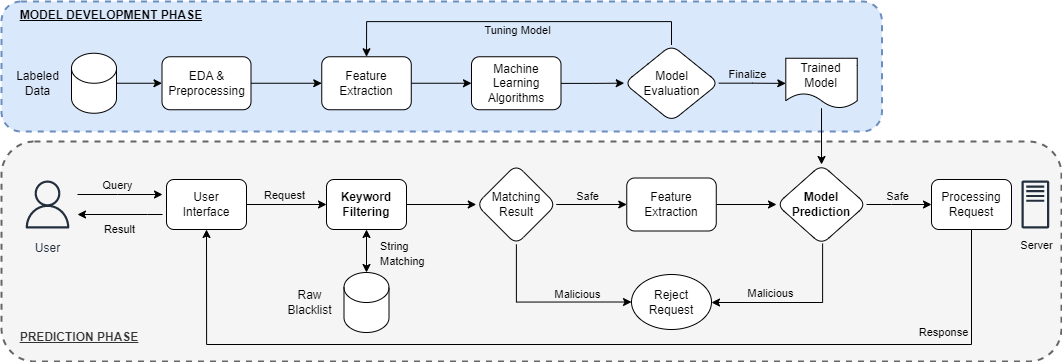
\includegraphics[width=.82\textwidth]{image/SQLI-Final.drawio.png}
  \caption{Design Workflow}
  \label{fig:proposed-workflow}
\end{figure*}

\par Figure \ref{fig:proposed-workflow} shows our proposed design, which separates the workflow into two phases. The model development phase aims to build a machine-learning model with the best predictive performance and the least prediction time. In the prediction phase, we implement the two-step prevention approach by combining keyword filtering and model prediction to prevent SQLi attacks.

\par The first step of the model development phase is to gather labeled data and an indicator of whether it is a malicious or safe query. Exploratory Data Analysis (EDA) is performed to understand the data better and decides the appropriate hyperparameters for the model. Preprocessing refers to the query cleansing step. Below, we provide an example of a query being cleansed consecutively:

\begin{itemize}[
    \setlength{\IEEElabelindent}{\dimexpr-\labelwidth-\labelsep}% Wrapping of text beyond first line of \item
    \setlength{\itemindent}{\dimexpr\labelwidth+\labelsep}% identation for each new \item
    \setlength{\listparindent}{\parindent}% Restore regular paragraph indentation
  ]
  \item Case folding: convert all text queries to lowercase since uppercase, and lowercase tokens have the same meaning. Example: 23" and 65 = 65 || chr (113) and "0x77" like "0x77
  \item Punctuation padding: insert white space before and after each punctuation to separate from alphanumeric characters, and each punctuation can be treated as one token. Example: 23 " and 65 = 65 | | chr ( 113 ) and " 0x77 " like " 0x77
  \item Numeric mapping: numeric values are too specific to be considered a single token, so they are mapped into each corresponding tag. There are three tags: <NUM> for regular numeric, <HEX> for hexadecimal, and <ASCII\_DEC> for a numeric followed by a char function. Example: <NUM> " and <NUM> = <NUM> | | chr ( <ASCII\_DEC> ) and " <HEX> " like " <HEX>
  \item Tokenizing: split the cleaned query into a list of tokens, using a single space as the separator. Example result: 19 tokens
\end{itemize}

\par The cleaned queries are converted into vector representation so that the model can compute numerically. The feature extraction technique for machine learning is TF-IDF, while a regular embedding layer is used for deep learning. The features are then fitted into several supervised machine learning algorithms (including LSTM). The model is evaluated using cross-validation and fine-tuned by adjusting the hyperparameters until it is optimized enough in terms of predictive performance and prediction time.

\par During the prediction phase, the query input by the user is matched to the static raw blacklist in the database. The user's request is considered malicious if a match is found in the blacklist. If it is considered safe, it is continued as input to the machine learning model to be predicted. Notice that the exact feature extraction step still has to be performed to represent the query using vector representation. The server will reject the user's request if the model predicts the query is malicious. If the query passes both keyword filtering and model prediction, the server will process it and return the result to the user via the user interface. The decision-making during this phase can be summarized using a logical OR operator shown in Table \ref{tab:decisionmaking}.

\begin{table}
  \caption{Decision making during the prediction phase}
  \label{tab:decisionmaking}
  \centering
  \begin{tabular}{lll}
    \toprule
    Keyword Filtering & Model Prediction & Final Decision  \\
    \midrule
    Malicious      & Malicious      & Malicious     \\
    Malicious      & Safe      & Malicious     \\
    Safe      & Malicious      & Malicious     \\
    Safe      & Safe      & Safe     \\
    \bottomrule
  \end{tabular}
\end{table}